\chapter{Archictetures for dialog}\label{architectures}


\section{1}

\section{2}

\section{3}

\section{4}

\section{Deep Reinforcent Learning}

In the paper \textit{Deep Reinforcement Learning for Dialogue Generation} \cite{Li:2016} the authors notice that since seq2seq models are trained by predicting the next sentence in a given conversation using the maximum-likelihood estimation (MLE) objective function, the model tends to generate  highly generic responses such as "\textit{I don't know}". This kind of responses creates conversation with little or no informational content. For example, the author let two agents talk and find some unsatisfactory results:

\begin{quote}
\begin{itemize}
\item[] A) how old are you?
\item[] B) I'm 16
\item[] A) 16?
\item[] B) I don't know what are you talking about.
\item[] A) You don't know what are you saying.
\item[] B) I don't know what are you talking about.
\item[] A) You don't know what are you saying.
\item[] $\dots$
\end{itemize}
\end{quote}

With that in mind the authors propose adding a rewarding signal to to guide the agent towards more meaningful responses, and formulate the dialog problem such that it is possible to model the long term influenced of a utterance. They choose the theoretical framework of reinforcement learning to achieve that.

\par This is a way to change the objective function that is being maximized during training. Instead of MLE objective, they try to learn a policy optimizing the long-term developer-defined reward from ongoing dialog simulations using policy gradient methods.

\par The authors are trying to combine two traditions of research in dialog generation, the one that sees dialog generation as a translation problem (the program should translate one utterance in a response); and the other that are focused in task oriented dialogs, an agent that utter a sentence is view as an agent that need to take action in an environment. This second tradition models the dialog task as a reinforcement learning problem. 


\par In this paper the learning system is described as follows: there are to agents A and B. They take turn talking with each other. So a dialogue can be represented as the sequence: $p_1, q_1, p_2, q_2, \dots, p_i, q_i$ where $p$ and $q$ are the sentences uttered by A and B, respectively.

\par For any agent, and \textbf{action} $a$ is a sentence. Since sentence can have any length, the action space is infinite.

\par A \textbf{state} is a pair $(p_i, q_i)$ of the previous two dialogue turns.

\par A stochastic policy $\pi(a|s)$ takes the form of an LSTM encoder-decoder $P(p_{i+1}|p_i, q_i)$.

\par The reward system in this setup have many parts. i) \textbf{Ease of answering}  the first part of the reward is the signal for \textit{forward-looking}, i.e., the agent should be punished if he produce sentences that do not move the the conversation forward. Using a set of $S$ of sentences such as 'I don't know what you are talking about', 'I have no idea', etc. and a Seq2Seq model $p_{Seq2Seq}$, a reward signal is calculated as

\begin{equation}
r_1 = - \frac{1}{N_{S}} \sum_{s\in S} \frac{1}{N_{s}} \log p_{Seq2Seq}
\end{equation}

where $a$ is an action (a sentence) $N_{S}$ is the cardinality of $S$ and $N_{s}$ is the number of tokens in the dull sentence $s$.

ii) \textbf{Information Flow} the authors penalize semantic similarity (cosine similarity) between consecutive turns form the same agent. Let $p_i$ and $p_{i+1}$ be two consecutive turns and $h_{p_{i}}$ and $h_{p_{i+1}}$ be the respective representation obtained form the encoder, them the reward signal $r_2$ is defined as the negative log of the cosine similarity:

\begin{equation}
r_2 = - \log \frac{h_{p_{i}} h_{p_{i+1}}}{||h_{p_{i}}|| ||h_{p_{i+1}}||}
\end{equation}


iii) \textbf{Semantic Coherence} the authors also consider the mutual information between the action a and previous turns in the history to ensure the generated
responses are coherent and appropriate:

\begin{equation}
r_3 = \frac{1}{N_{a}} \log p_{Seq2Seq}(a| q_i, p_i) + \frac{1}{N_{q_{i}}} \log p_{Seq2Seq}^{backward}(q_i| a)  
\end{equation}

where $p_{Seq2Seq}(a| p_i, q_i)$ denotes the probability of generating
response a given the previous dialogue utterances $[p_i, q_i]$. $p_{Seq2Seq}^{backward}(q_i| a)$ denotes the backward probability
of generating the previous dialogue utterance $q_i$ based on response $a$.

And so the reward for action $a$ is:

\begin{equation}
r(a, [p_i, q_i]) = \lambda_1 r_1 + \lambda_2 r_2 + \lambda_3 r_3
\end{equation}

where $\lambda_1 + \lambda_2 + \lambda_3 = 1$ (the authors have used $\lambda_1 = 0.25, \lambda_2 = 0.25, \lambda_3 = 0.5$.

\par First the autors have trained the Seq2Sqeq model on the OpenSubtitles dataset; the treat each turn in the dataset as a target and the concatenation of two previous sentences as source inputs. they use this trained model to train a mutial information model. This last model is the one that they use to initialize the policy model $p_{RL}$.

\par In this context an episode is a simulate conversation between two agents ($A$ and $B$). At the initial step a message from the training set is fed to $A$. Using an encoder -decoder model, $A$ encodes the message and decode a set of responses to $B$. In its turn, $B$ combines the set of immediate output of $A$ with the dialog history and using the encoder-decoder model generates a set of responses. These responses are feeded to $A$, and the process continues. Figure \ref{MDPConver} shows one visualization of this process. Each played action is considered a \textit{turn}. There are two stopping criteria: one of the agents generate dull responses like "I don't know" or two consecutive responses from the same agent are highly overlapping (i.e., they share more than $80\%$ of their words).


\begin{figure}[ht!]
\label{MDPConver}
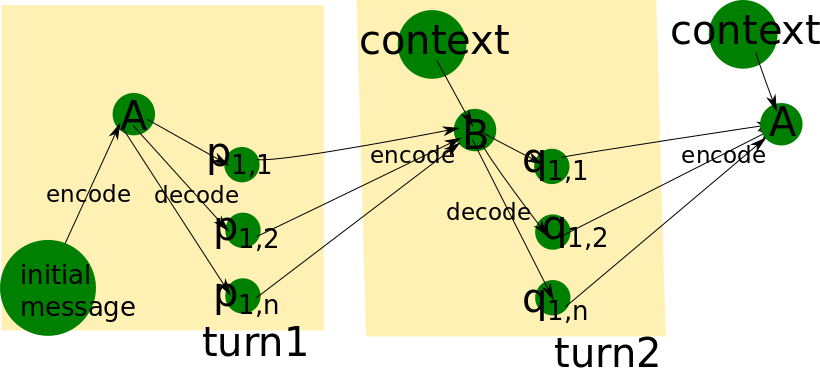
\includegraphics[width=5cm]{img/MDPconversation_placeholder.png}
\caption{MDP conversation}
\end{figure}

\par The authors use policy gradient methods to search a model to maximize the expected future reward:

\begin{equation}
J_{RL}(\vect{\theta}) = \E_{p_{RL}(a_{1:T})} \left[\sum_{i=1}^{T} R(a_i, [p_i, q_i]) \right]
\end{equation}

where $R(a_i, [p_i, q_i])$ denotes the reward resulting from action $a_i$. The gradient is estimated by the \textit{likelihood ratio trick}:

\begin{equation}
\grad{\vect{\theta}}{J_{RL}} \approx \sum_{i} \grad{\vect{\theta}}{p(a_{i} | p_{i}, q_{i})} \sum_{i=1}^{T}R(a_i, [p_{i}, q_{i}])
\end{equation}

\par Three different metrics are used: i) \textit{length of the dialog} -- average number of simulated turns; ii) \textit{degree of diversity} -- number of distinct unigrams and bigrams in generated responses; iii) \textit{human evaluation}.

\par The paper compare three models: Seq2seq, mutual information and the proposed model using reinforcement learning (RL model). The RL model have a slightly better score then the mutual information model in i) and ii). But in iii) human judges are presented with simulated conversation between the two agents, some conversation were generated by the RL model and some were generated by the mutual information model. The judges voted in which one is the better (ties are permitted).  The RL model win $72\%$ of time, lose $12\%$ of time and tie $16\%$ of time.

\section{How to evaluate dialogs?}

wewewe
\subsubsection{BLUE}
This metric was proposed in \cite{Papineni2001} for automatic translation. It compares n-grams (up to 4) of the candidate translation with the n-grams of the reference translation and count the number of matches; it also ads brevity penalty for too short translations. The formula for this metrics is:

\begin{equation}
BLUE = min \left(1, \frac{output-length}{reference-lenght} \right) \left(\prod_{n=1}^{4} precision_{n} \right)^{\frac{1}{4}}
\end{equation}

Where $precision_{n}$ is number of $n$-gram overlap between the candidate and the reference divided by the number of all $n$-grams in the candidate. BLUE scores ranges from $0$ to $1$. Typically this score is computed over an entire corpus and was originally designed for use with multiple reference sentences. To give one simple example we will use the following Portuguese sentence:

\begin{center}
`em plano aberto, a cidade parece linda'
\end{center}

The reference translation is

\begin{center}
`in a wide shot, the city looks beautiful'
\end{center}

Now consider two candidates:

\begin{center}
$c_1$: `in the open, the city looks beautiful'\\
$c_2$: `in open plan, the city looks gorgeous'\\
\end{center}

\begin{figure}
\label{bluetable}
\begin{center}
\begin{tabular}{|c|c|c|}
\hline
\cellcolor{blue!10} Metric& \cellcolor{blue!10} $c_1$ & \cellcolor{blue!10} $c_2$ \\ \hline
\cellcolor{blue!10} $precision_1$& $5/7$ & $4/7$ \\ \hline
\cellcolor{blue!10} $precision_2$& $3/6$ & $2/6$  \\ \hline
\cellcolor{blue!10} $precision_3$& $2/5$ & $1/5$  \\ \hline
\cellcolor{blue!10} $precision_4$& $1/4$ & $0/4$  \\ \hline
\cellcolor{blue!10} brevity penalty& $7/8$ & $7/8$  \\ \hline
\cellcolor{blue!10} $BLUE$& $0.38$ & $0$ \\ \hline
\end{tabular}
\end{center}
\end{figure}


Table \ref{bluetable} shows the precision for each $n$-gram (up to $4$) and the BLUE score for each candidate.



\subsubsection{Automatic Turing test}

The authors of \cite{Lowe:2016} defend that the Turing Test \cite{Turing} provides one accurate automatic evaluation procedure for dialog systems. But the test need to be changed in order to avoid human evaluation. Theirs basic assumption is that : \textit{a good chatbot is one whose responses are score highly on appropriateness by human evaluators}. So they collected a dataset of appropriateness scores to various dialogues responses; with this dataset they have trained a model (called automatic dialogue evaluation model - ADEM) to predict human scores.

\par The dataset contains $4104$ conversational responses confectioned on dialog contexts and human judgments (scores). The context is from the Twitter Corpus and the responses are generated by different models (these are also human-generated responses but they are not the ones from the original corpus).

\par BLEU is a metric to compute word overlap. It is normally used for automatic translation. It can be used to dialogue response evaluation but it fail in capturing the semantic similarity between the model and reference responses. And since this method compares only the model's output and the reference response, it does not consider the context of the conversation.

\par ADEM is a hierarchical RNN encoder. Given the dialogue context $c$, reference response $r$ and model response $\hat{r}$ ADEM encodes each one of them into a vector ($\vect{c}, \vect{r}$ and $\vect{\hat{r}}$ respectively) and computes the following score:

\begin{equation}
score(c,r,\hat{r}) = \frac{(\vect{c}^{T} \vect{M} \vect{\hat{r}} + \vect{r}^{T} \vect{N} \vect{\hat{r}} - \alpha)}{\beta}
\end{equation}

\par The matrices $\vect{M}$ and $\vect{N}$ map the model response $\vect{\hat{r}}$ into the space of contexts and reference responses, respectively. The model gives high scores to responses that have similar vector representations to the context and reference response after this projection. The model is trained in order to minimize the squared error between the model prediction and the human score with L2-regularization:

\begin{equation}
J(\vect{M}, \vect{N}) = \sum_{i}^{K}[score(c,r,\hat{r}) - human_{i}]^{2} + \gamma (||\vect{M}||^2 + ||\vect{N}||^2)
\end{equation}

\par To have a good encoder, the authors pre-trained the model (only the parameters of the encoder) using a dialogue model, more specifically a latent variable hierarchical recurrent encoder-decoder (VHRED) model.

\par Using this model the authors obtained a good correlation between ADEM and the human judgment. The model is often very good at assigning low scores to poor responses, but it tends to be too conservative because the model learns to predict scores closer to the average human score. 

\par The authors notice that the metrics from \cite{Li:2016} are based on hand-crafted features and it is unclear whether such objectives are preferable over retrieval-based cross-entropy or word-level log-likelihood objectives. They also notice that current dialogue  systems are incapable of generating responses that are rated as highly appropriate by humans.
